% ---------------------------- comment out when compiling the full document -------------------
\documentclass[twoside,11pt]{article}  % default square logo 
\usepackage{amssymb}
\usepackage{caption}
\usepackage{upgreek}
\usepackage{subfig}
\usepackage{textcomp}
\usepackage{graphicx}


\begin{document}
\baselineskip=15pt
% ---------------------------------------------------------------------------------------------------------------

\begin{figure}[!t]
\centering
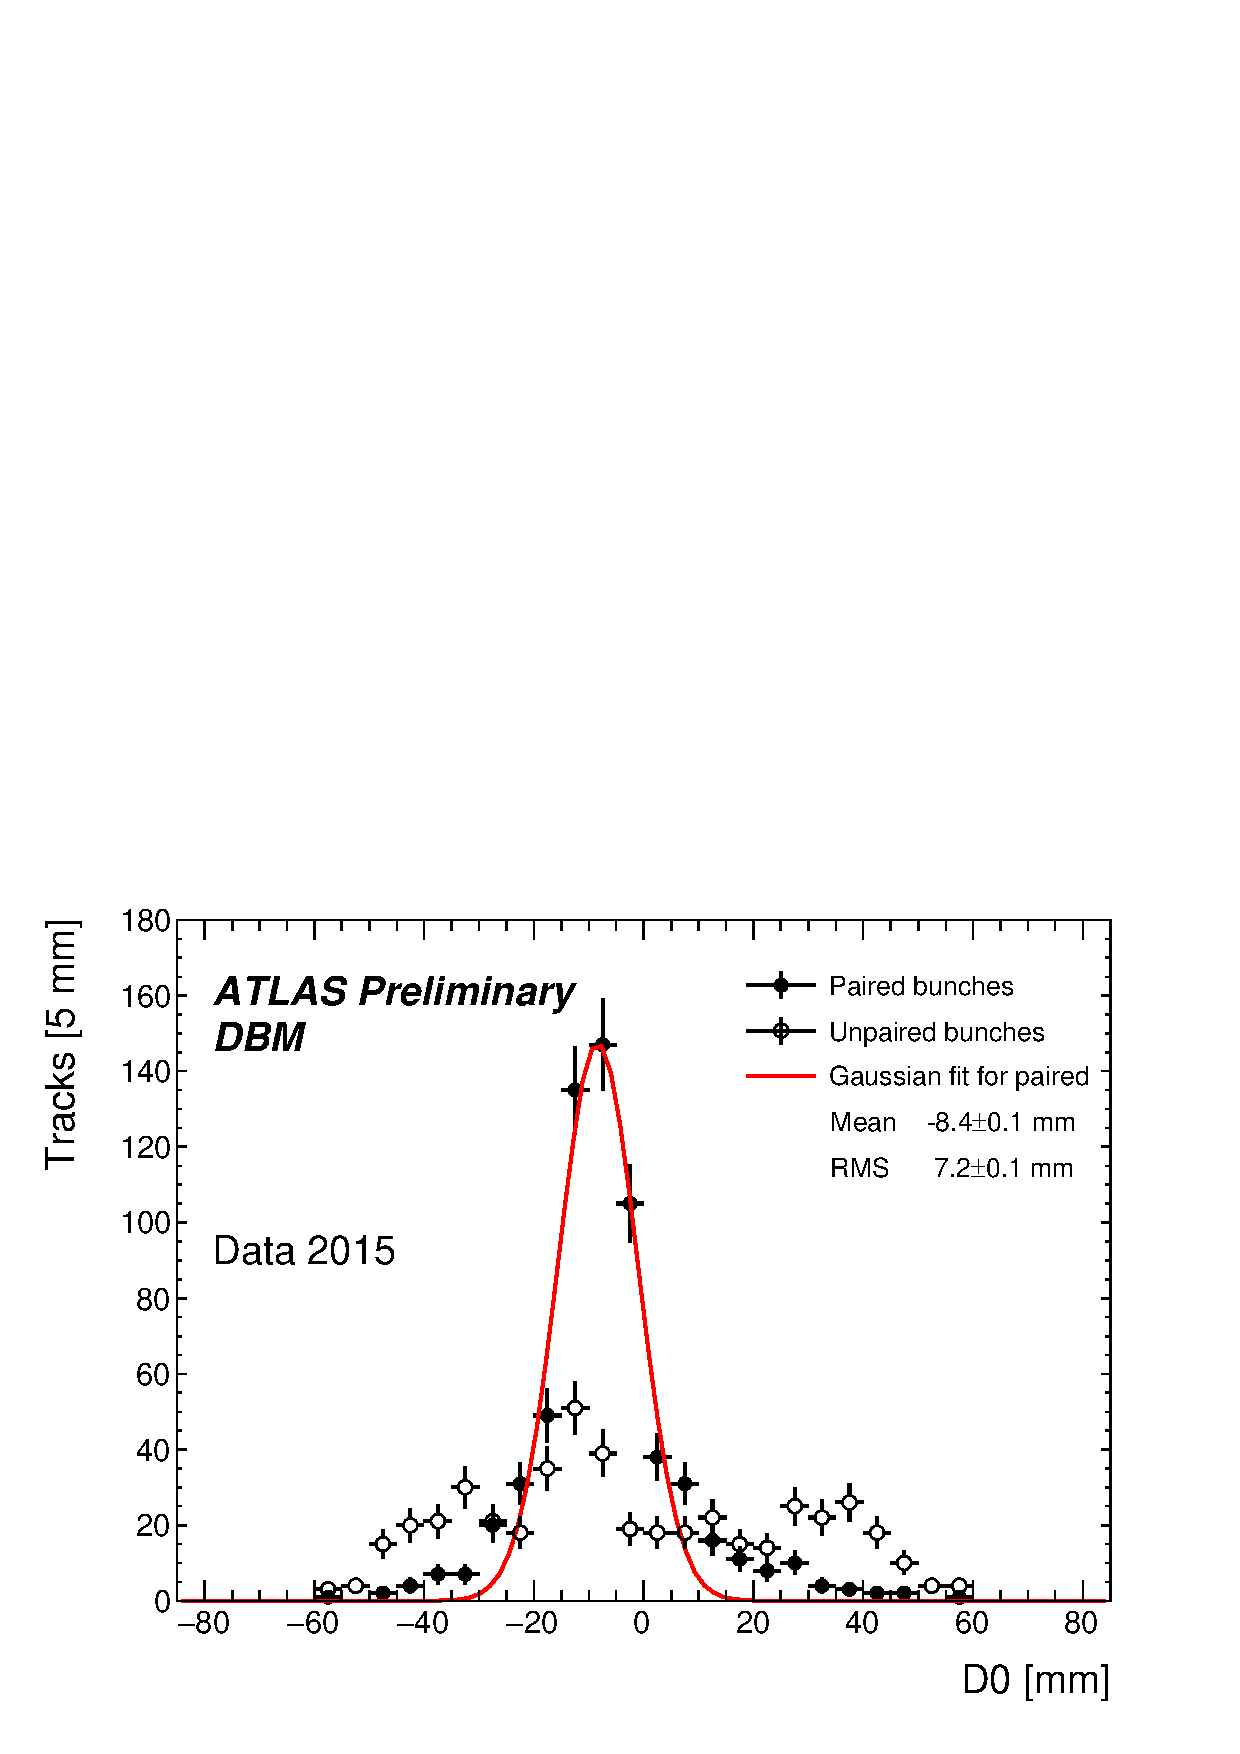
\includegraphics[width=0.8\textwidth]{D0.pdf} \label{}
\caption{Radial distance of the closest approach of the projected particle tracks to the interaction point as recorded by a single DBM telescope. The Gaussian fit yields a D0 with a mean of -8.4~mm and an RMS of 7.2~mm. No alignment has yet been included. The two side peaks of the tracks in the distribution for the tracks with unpaired bunches correspond to secondary particles created by collisions of protons with the pipe and the surrounding material. Data acquired during one run in July 2015.}
\end{figure}

\begin{figure}[!t]
\centering
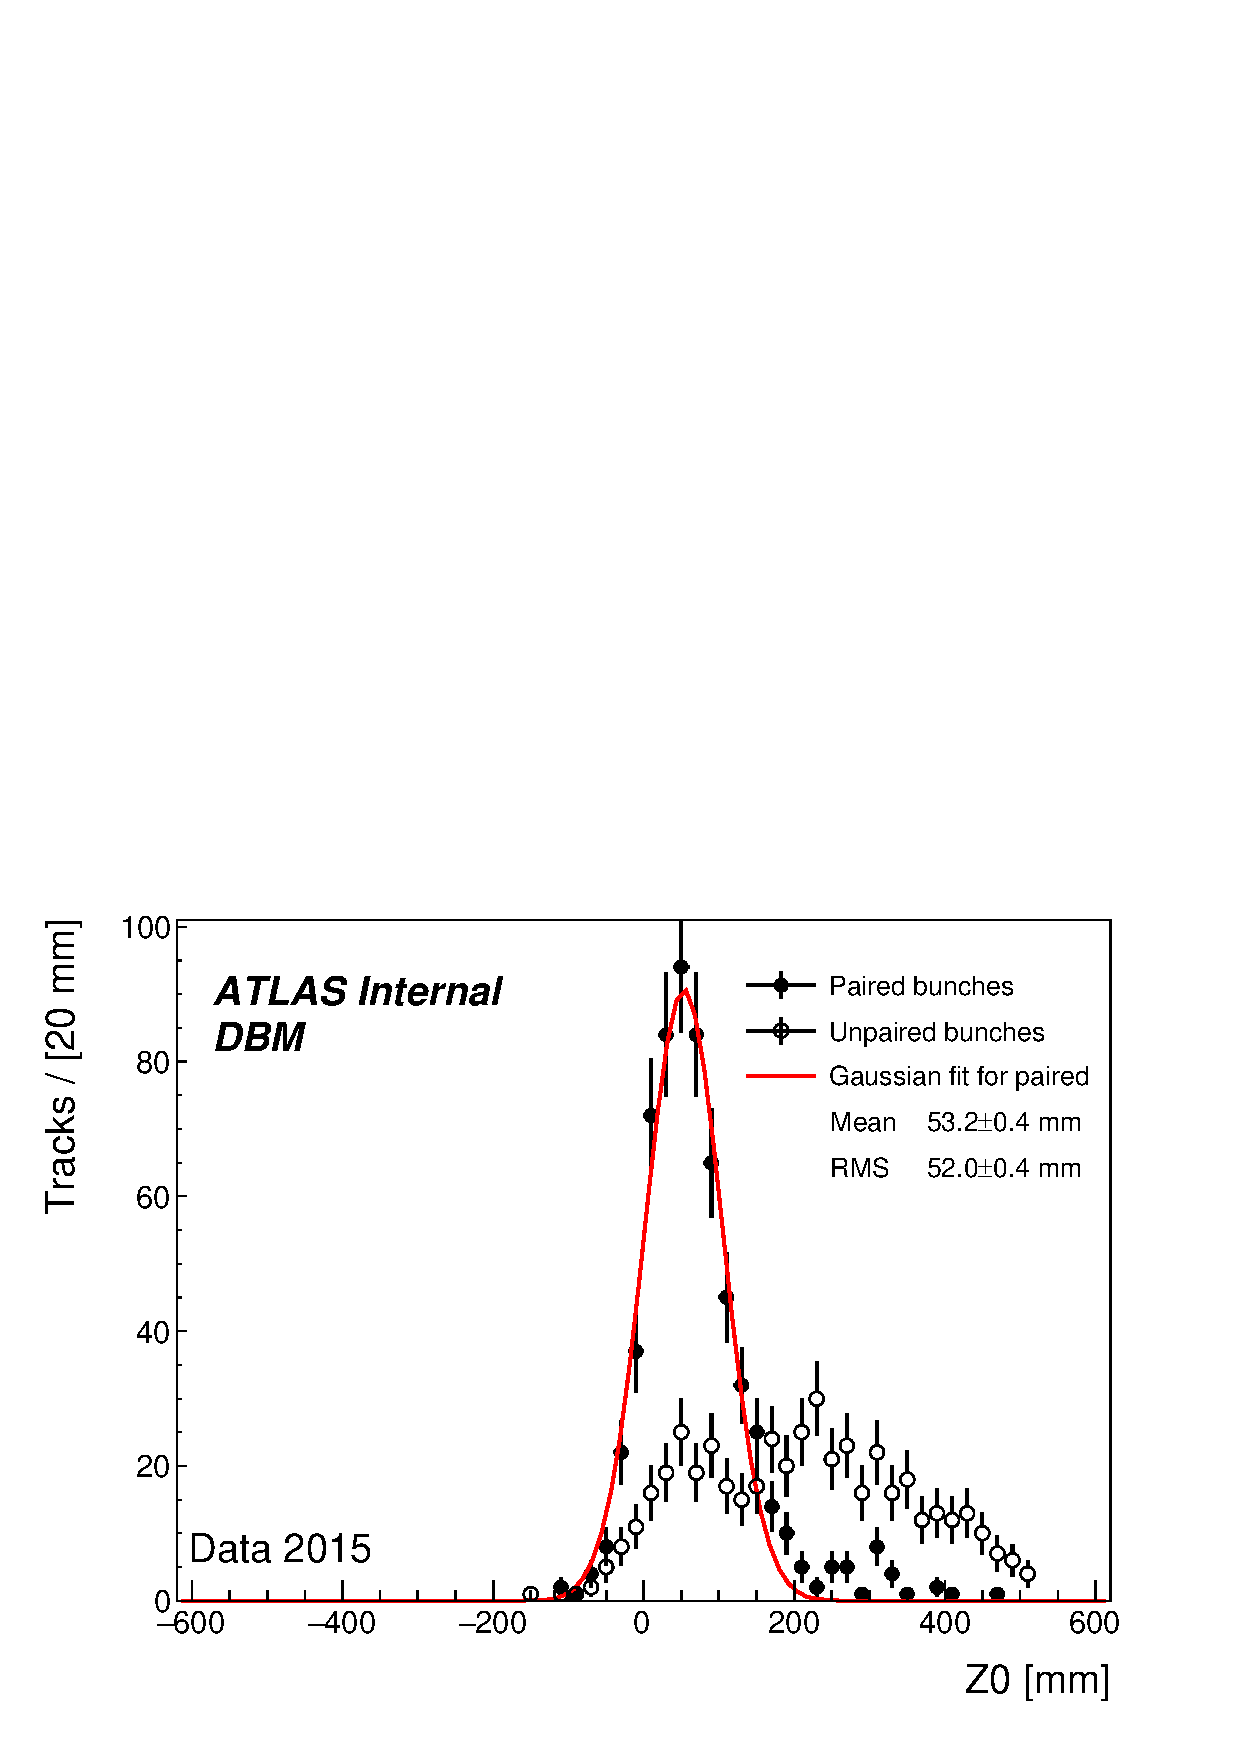
\includegraphics[width=0.8\textwidth]{Z0.pdf} \label{}
\caption{Longitudinal distance of the closest approach of the projected particle tracks to the interaction point as recorded by a single DBM telescope. The Gaussian fit yields a Z0 with a mean of 53.2~mm and an RMS of 52.0~mm. No alignment has yet been included. Data acquired during one run in July 2015.}
\end{figure}

% ---------------------------- comment out when compiling the full document -------------------
\end{document}
% ---------------------------------------------------------------------------------------------------------------
